\documentclass{report}
\usepackage{hyperref}
\usepackage{tikz}
\usetikzlibrary{positioning}
\usepackage{extensions/tikz-uml}
\usepackage{xcolor}
\usepackage{float}
\usepackage{notoccite}
\usepackage{titlesec}
\usepackage{etoolbox}
% for header and footer
\usepackage[a4paper, margin=1in, headheight=16pt]{geometry}  % Ensures enough space for header

% Header/Footer setup
\usepackage{fancyhdr}
\pagestyle{fancy}
\fancyhf{}  % clear all headers and footers
\renewcommand{\sectionmark}[1]{\markright{#1}}
% Define a command to set up = header/footer 
\newcommand{\myfancysetup}{
  \fancyhead[L]{Henry Field - Computer Science NEA}
  \fancyhead[R]{\rightmark}
  \fancyfoot[L]{Candidate Number: \textbf{1749}\\Center Number: \textbf{58231}}
  \fancyfoot[R]{Page \thepage}
  \renewcommand{\headrulewidth}{0.4pt}
  \renewcommand{\footrulewidth}{0pt}
}
% Apply the setup to both 'fancy' and 'plain' page styles
\myfancysetup
\fancypagestyle{plain}{\myfancysetup}


\usepackage[
    backend=biber,
    style=numeric,
    sorting=none,
    sortcites=true,
    date=comp,
    urldate=long
]{biblatex}

\addbibresource{References.bib}
\begin{document}

\title{NEA: Disease Spread Simulation}
\author{Henry Field}
\date{\today}
\maketitle
\setcounter{tocdepth}{5}
\tableofcontents
\newpage
\chapter{Analysis}
\section{Introduction to the Problem}
Understanding how infectious diseases spread through urban environments is a complex and urgent problem, especially in light of recent global health crises. During pandemics, decision-makers rely on accurate models to evaluate the effectiveness of public health interventions such as social distancing, lockdowns, and vaccination. However, many existing simulations operate at national or global scales, often lacking the granularity needed to inform decisions at the community level.

This project seeks to address this gap by simulating disease spread within a city-sized environment, consisting of approximately 100,000 agents (representing individuals) and 20,000 nodes (representing buildings or gathering points). The problem being tackled is how to model and visualize disease transmission within a realistic, localized setting, so that the impact of specific strategies (e.g., closing schools or limiting public transport) can be analyzed.

The aim is to design and implement a simulation that accurately reflects how a disease could spread through a densely populated urban area, based on various parameters such as agent mobility, infection rate, and building density. The solution will not only allow for analysis of intervention strategies, but also provide a clear, visual representation of disease progression over time—making the data accessible and informative for both experts and the general public.

This project combines elements of agent-based moddelling, data visualization, and algorithmic design to address a real-world problem through computational means.

\section{Client}
\subsection{Introduction of client}
The primary client to my software would be a clinical researcher / policymaker who is looking to implement changes that would protect their population from harm through the spread of disease. I was fortunate to visit the Imperial university Department of Infectious diseases and to speak with both a researcher and a software developer there to discuss my projects objectives and collect their initial thoughts. They were highly supportive of my ideas and provided great insight into some methods I could try and some architectural considerations I should make. Unfortunately I will likely be unable to remain in continuous contact with them over the project's development so I collected their initial thoughts and am potentially looking to be able to get some contacts at Cambridge based research facilities who I can be in more frequent communication with.

The faculty at Imperial gave me a loose brief from which I can expand, the software should:
\begin{itemize}
    \item Give users a space to simulate disease spread in a city
    \item work on an agent by agent basis for a realistic disease spread
    \item Utilise real map data for location based modelling
    \item Utilise population data for accurate agent generation
\end{itemize}

A secondary Client to my software would be members of the general public who want to easily visualise the impact very small measures (such as face coverings or self-isolation) can make to the larger picture. By making my software very intuitive even to those without scientific it can used to quickly visualise and prove a point to others. A variety of my family members and family friends (from a variety of academic backgrounds including biologists) have agreed to test my software and provide feedback on its usability and intuitiveness. I will also be able to use their feedback to improve the software's accessibility for those without a scientific background.

\subsection{Client Interview}

\begin{center}
    \textbf{Interview With x: Q \& A}
\end{center}



\begin{description}
    \item[Q:] What is the main goal you would like this simulation software to achieve?
    \item[A:] The main goal is to provide a tool that can simulate disease spread at a city level, allowing us to test the impact of different interventions and policies in a realistic, data-driven environment.

    \item[Q:] What features are most important for your research or decision-making?
    \item[A:] The ability to use real map and population data, simulate individual agent behaviours, and visualize the effects of interventions like school closures or mask mandates are essential. Clear, accessible output is also important for communicating results.

    \item[Q:] What challenges do you face with current modelling tools?
    \item[A:] Most existing tools are either too broad in scope (national/global) or too technical for non-experts. They often lack flexibility, detailed local modelling, or require significant programming expertise.

    \item[Q:] How important is accessibility for non-expert users?
    \item[A:] Very important. Policymakers and the public need to understand the results without needing a technical background. Intuitive interfaces and clear visualizations are key.

    \item[Q:] What data sources do you recommend for agent and location generation?
    \item[A:] OpenStreetMap for geographic data and ONS for population demographics are good choices. Disease parameters should be customizable, with presets for common scenarios.

    \item[Q:] How would you measure the success of this software?
    \item[A:] Success would be measured by its ability to accurately simulate scenarios, provide actionable insights, and be usable by both researchers and the public. Validation against real-world data and positive feedback from experts would be ideal.
\end{description}


\section{Problem Research}
With the focus of my project being academic in nature and having a smaller userbase than e.g. a social media app I knew I would have to focus my search for user issues before beginning any software development. To start I researched the current offerings available to professionals in this industry, these mostly exist in two forms: complete graphical software packages and computational models / algorithms, here are the packages I researched:
\subsection{Existing Software}
\subsubsection{Gleamviz}
GLEaMviz (Global Epidemic and Mobility Model) is a computational tool designed to simulate the spread of infectious diseases on a global scale by integrating real-world data on population, human mobility, and disease dynamics. It combines a metapopulation approach—dividing the world into subpopulations connected by transportation networks—with stochastic compartmental models (e.g., SEIR) to simulate disease progression and transmission. By incorporating airline travel, commuting patterns, and demographic information, GLEaMviz enables researchers and public health officials to model outbreak scenarios, assess intervention strategies, and predict potential epidemic outcomes with spatial and temporal precision.

\begin{figure}[H]
    \centering
    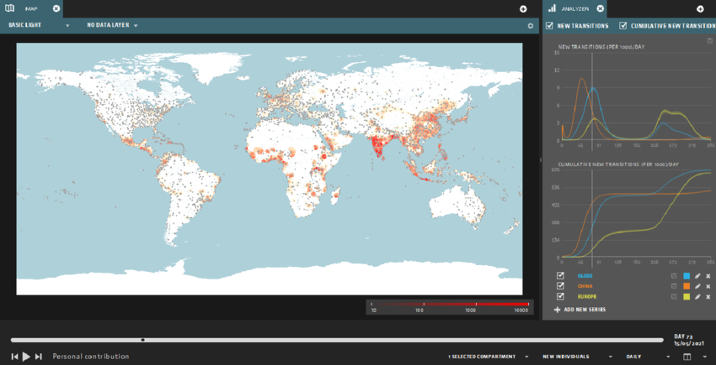
\includegraphics[width=0.7\textwidth]{Chapters/AnalysisMedia/Gleamviz.png}
    \caption[GLEaMviz simulation interface]{Screenshot of the GLEaMviz simulation interface \autocite{GLEAMvizGlobalEpidemic}}
    \label{fig:gleamviz}
\end{figure}

Pros
-	Integrates global mobility
-	Built in SEIR (susceptible-exposed-infected-recovered) modelling
-	Intuitive GUI
-	Robust global simulation	-	Limited spatial resolution for city/village level modelling
Cons
-	Closed source and inflexible
-	Can't simulate detailed intervention modelling


\subsubsection{AnyLogic}
AnyLogic is a commercial simulation platform that supports multiple modelling paradigms, including agent-based, system dynamics, and discrete-event simulation. Its flexibility allows users to build detailed models of epidemics within cities, hospitals, or regions, integrating individual behaviour, mobility, and interventions. AnyLogic is popular in industry and academia for its visual interface, GIS support, and ability to simulate scenarios involving healthcare logistics or policy interventions. While powerful, its more advanced features require a commercial license and technical expertise.

\begin{figure}[H]
    \centering
    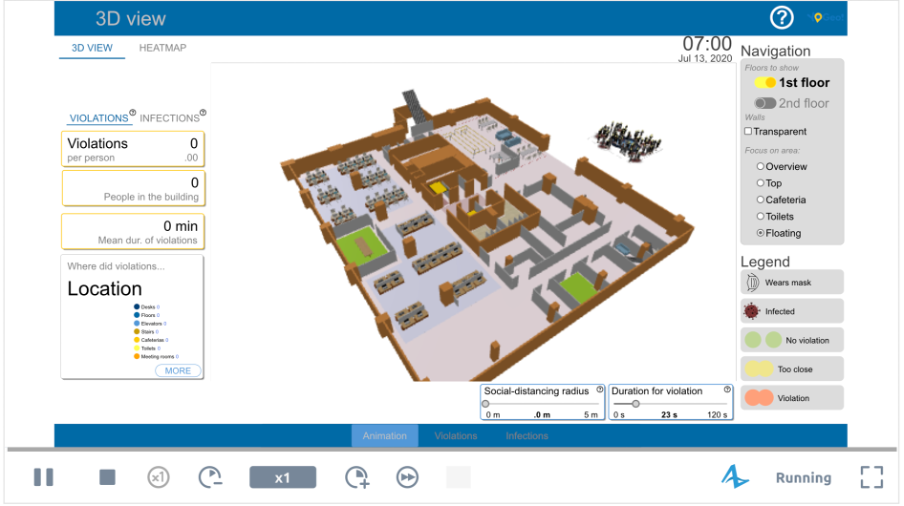
\includegraphics[width=0.7\textwidth]{Chapters/AnalysisMedia/AnyLogic.png}
    \caption[GLEaMviz simulation interface]{Screenshot of the Anylogic interface simulating an office floor \autocite{AnyLogicCOVID19Simulation2022} }
    \label{fig:anylogic}
\end{figure}

Pros
-	Powerful agent-based modelling platform
-	Simple and customisable GUI
-	Accurately models small areas such as within a store or even a room
Cons
-		-	Steep learning curve for project setup
-	Commercial licence required
-	Can’t simulate areas larger than a small village

\subsubsection{Covid-19 scenarios (Neher Labs)}
COVID-19 Scenarios is an interactive web-based tool created by the Neher Lab for simulating the spread of COVID-19 using a configurable SEIR model. Users can adjust key parameters like R0, hospitalization rates, and intervention timing to explore different pandemic scenarios and healthcare outcomes. While not a full simulation engine, it provides a quick and intuitive way for policymakers and the public to visualize the impact of control measures. Its simplicity and focus on COVID-19 make it accessible but limited in scope and adaptability.

\begin{figure}[H]
    \centering
    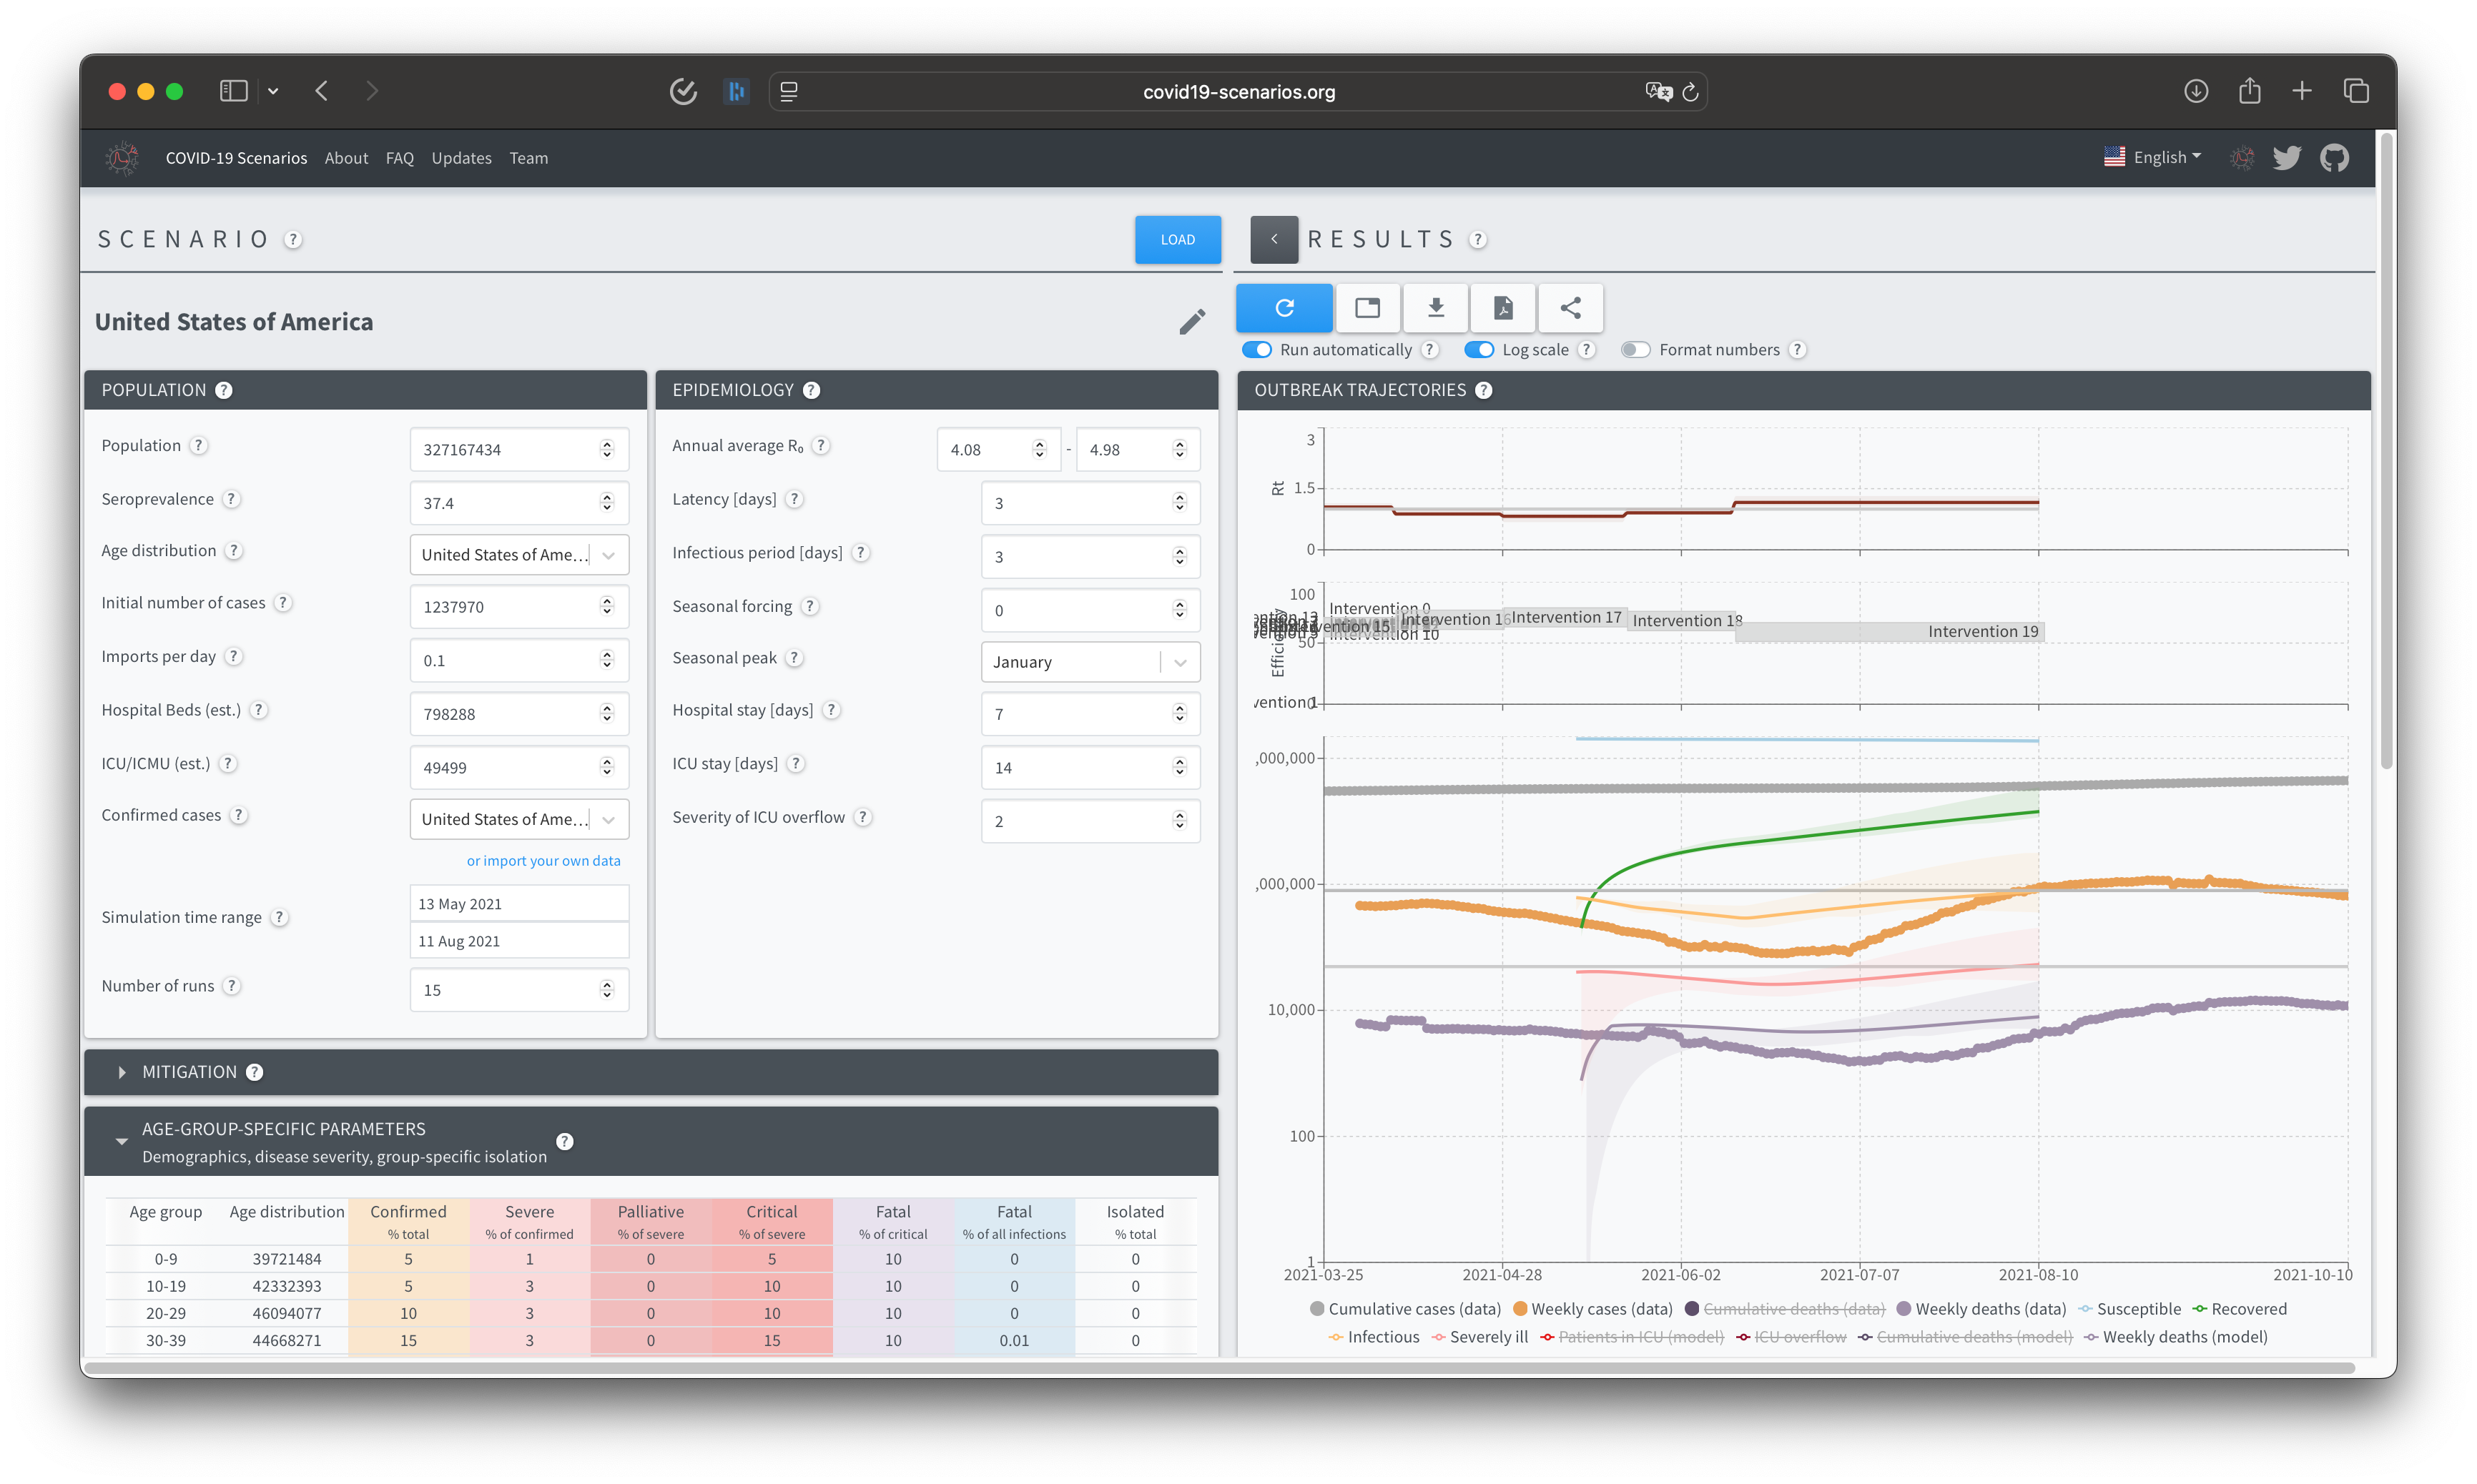
\includegraphics[width=0.7\textwidth]{Chapters/AnalysisMedia/Covid19Scenarios.png}
    \caption[]{Screenshot of the Neher Labs Anylsis system \autocite{COVID19Scenarios} }
    \label{fig:Covid-19scenarios}
\end{figure}


\subsubsection{FRED (Fast Epidemiological Dynamic Simulator)}
FRED is an agent-based epidemic modelling system developed by the University of Pittsburgh, designed to simulate infectious disease transmission at the individual level using real census data and synthetic populations. It allows detailed modelling of social contact patterns within households, schools, workplaces, and communities, making it ideal for city-level or regional policy planning in the United States. FRED supports a wide range of disease models and interventions, though its geographic coverage is primarily US focused, and it requires some programming effort to customize.

\begin{figure}[H]
    \centering
    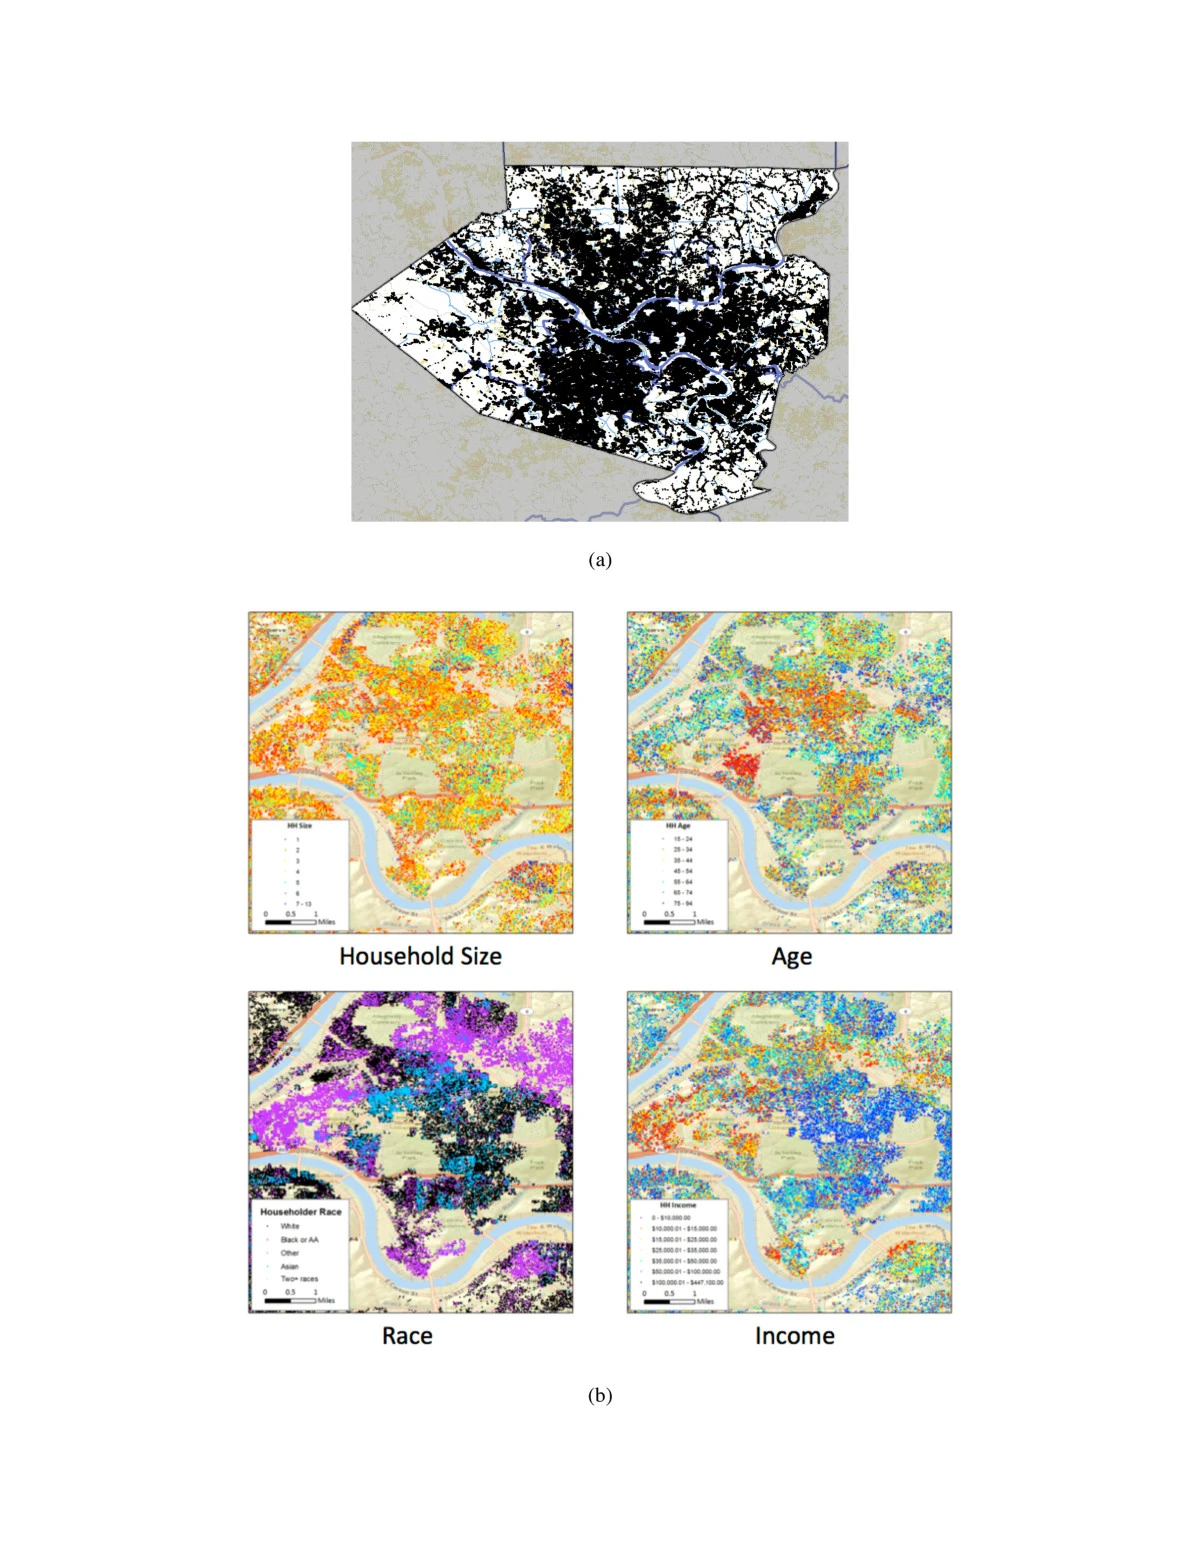
\includegraphics[width=0.5\textwidth]{Chapters/AnalysisMedia/FRED.png}
    \caption[]{Screenshot of the FRED interface \autocite{grefenstetteFREDFrameworkReconstructing2013} }
    \label{fig:fred}
\end{figure}
Pros
-	Agent based, fine scale model similar to what I’m trying to produce
-	Uses real census / demographic data from online government sources
-	Open source and extensible	-	U.S. centric and difficult to customise for other nations
Cons
-	Steep learning curve requiring programming
-	Very simplistic,  outdated interface
-	simulation appears random due to ‘popping in to view’


\subsubsection{EpiModel}
EpiModel is an open-source R package for simulating and analysing the spread of infectious diseases using deterministic, stochastic, and network-based compartmental models. It offers a flexible framework for modelling complex transmission dynamics, including sexual networks, social distancing, and other behavioural factors. EpiModel is well-suited for academic research and policy studies and allows users to build custom disease models with full control over parameters and structure. However, it requires proficiency in R and is not optimized for high-resolution spatial modelling.

\begin{figure}[H]
    \centering
    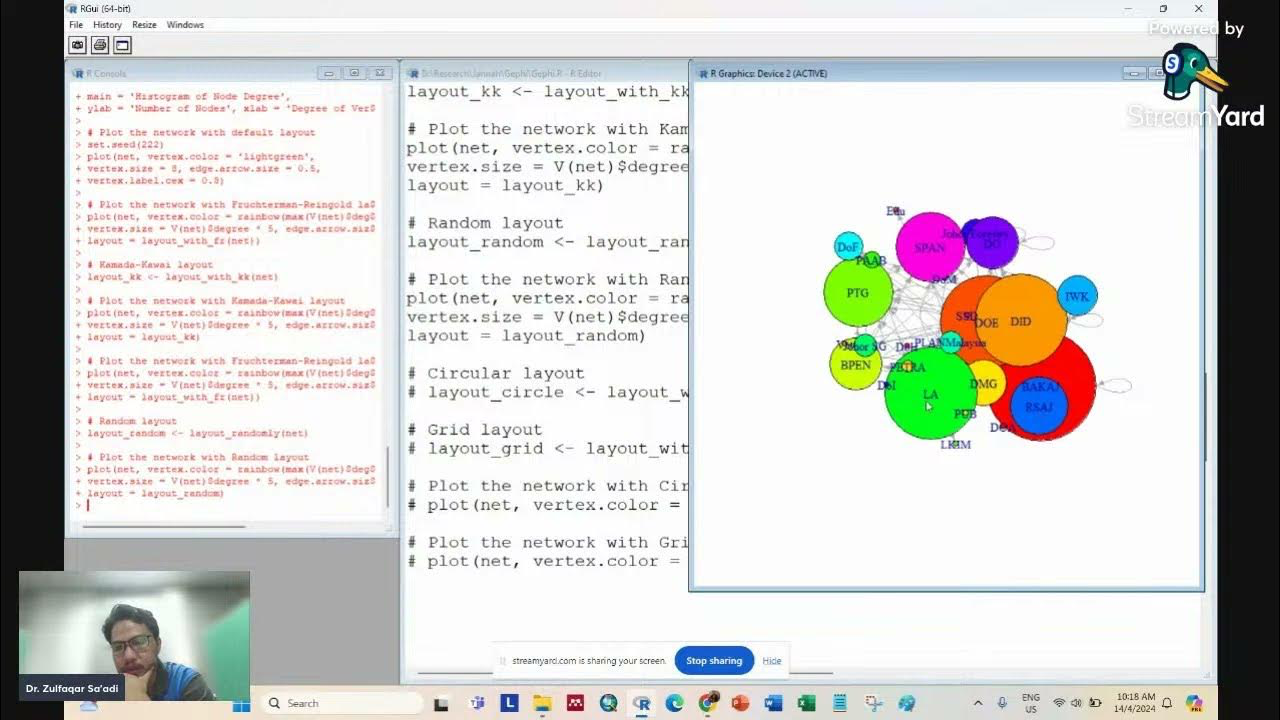
\includegraphics[width=0.7\textwidth]{Chapters/AnalysisMedia/EpiModel.png}
    \caption[]{An application of EpiModel \autocite{declassifiedmalaysiaUsingEpiModelIgraph2024}}
    \label{fig:EpiModel}
\end{figure}
Pros
-	Supports deterministic, stochastic, and network-based models
-	Highly Flexible and extensible
-	Great for research and education	-	Requires strong  programming skills to customise
Cons
-	Cant support GIS data or global mobility
-	No GUI available


\subsubsection{EpiSimdemics}
EpiSimdemics is a scalable, high-resolution agent-based modelling framework developed for simulating the spread of infectious diseases through detailed social contact networks. It models individual-level interactions across various locations such as homes, schools, and workplaces, allowing for fine-grained intervention testing like school closures or targeted quarantines. Designed for large urban areas or regional populations, it supports policy simulations with realistic behavioural components. However, its complexity and limited public accessibility make it more suitable for research collaborations than casual use.

\begin{figure}[H]
    \centering
    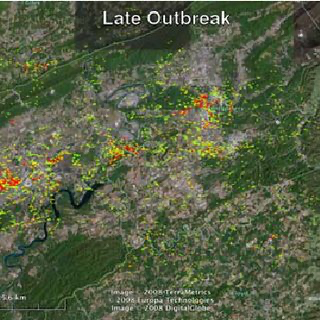
\includegraphics[width=0.4\textwidth]{Chapters/AnalysisMedia/EpiSimdemics.png}
    \caption[]{EpiSimdemics City Simulation \autocite{inproceedings}}
    \label{fig:EpiSimdemics}
\end{figure}

Pros
-	Large scale agent-based simulation (cities / counties)
-	Handles individual behaviours
-	Highly detailed results
Cons
-	No Gui for use / requires expert guidance / training	-	Complex setup
-	Not open source / limited to government use
-	High computational workload for resource


\subsubsection{OpenABM}
OpenABM-Covid19 is a lightweight, open-source agent-based simulation model tailored to study the effects of non-pharmaceutical interventions on COVID-19 transmission. Written in Python and grounded in demographic and mobility data, it simulates detailed contact patterns across households, workplaces, and public spaces. The model is designed to be transparent, easy to adapt, and useful for both researchers and policymakers. While currently COVID-specific, its modular structure allows adaptation to other diseases with some effort.
Pros
-	Open source
-	Well documented
-	Provides detailed intervention testing
-	Supports age structured population
Cons
-	Focused on covid-19
-	Requires coding skills (python)

\subsubsection{SimInf}
SimInf is an R-based modelling framework for simulating stochastic compartmental models (such as SEIR) in spatially structured populations. It is designed for speed and scalability, using C/C++ for backend computation while integrating with R for analysis and visualization. SimInf is particularly suited for scenarios involving many small subpopulations connected by movement or trade, such as livestock disease spread or localized outbreaks. It’s powerful for structured models but lacks agent-based or behaviour-driven simulation capabilities.
Pros
-	Fast simulations
Cons
-	Complex data analysis built in	-	Requires familiarity in C and R
-	Uses compartment model, not models so less accurate

\subsubsection{Flute}
FluTE is an agent-based epidemic model designed specifically to simulate the spread of influenza within structured populations, using realistic household, workplace, and school networks. It incorporates age-stratified interactions and intervention strategies like vaccination and antiviral distribution. Though originally built for U.S. populations, it can be adapted to other contexts with sufficient demographic data. FluTE is open-source and efficient but relatively rigid in scope, requiring C++ programming knowledge to modify or extend.
Pros
-	Agent based
-	Grounded on realistic demographic and household structures
-	Open source	-	Written in c++ and is hard to modify
Cons
-	Primarily US focused
\subsubsection{EMOD (Epidemiological MODelling software)}
EMOD is a flexible, open-source epidemiological modelling platform developed by the Institute for Disease Modelling. It supports highly detailed, agent-based simulations of diseases such as malaria, HIV, tuberculosis, and COVID-19, incorporating biological, environmental, and behavioural factors. EMOD is particularly strong in modelling vector-borne and sexually transmitted infections with age-structured and geographically targeted interventions. Though powerful, it has a steep learning curve and requires configuration via JSON files and scripting in Python or C++.
Pros
-	Very detailed agent-based disease modelling
-	Highly customisable transmission dynamics
-	Official tool from institute for disease modelling 	-	High barrier to entry needing configuration and code knowledge

Cons
-	Steeper learning curve
-	No GUI

Next I investigated some more context to understand the industry of epidemics and computational modelling:

\subsection{Epidemics Research}
Next I investigated some more context to understand the industry of epidemics and computational modelling:
\subsubsection{Agent Based Computational Modelling}{}
\textbf{Source:} \autocite{bissettAgentBasedComputationalEpidemiological2021}

The paper explores the use of agent-based models (ABMs) to simulate the spread of infectious diseases in human populations. It presents a modular framework that integrates synthetic population generation, contact network modeling, and disease transmission dynamics. By creating detailed, data-driven simulations of how individuals interact in households, schools, workplaces, and public spaces, the model allows for realistic analysis of disease spread. The paper emphasizes the scalability of their system, which is capable of simulating populations at city or even national scale, and highlights the importance of modeling localized interactions to understand how outbreaks evolve and respond to different interventions.

The paper especially highlights the difficulty of generating realistic populations as data can often be hard to come by. To tackle these challenges the researchers propose a more mathematical model that utilises randomness between known nodes / data to help facilitate the flow of a population in a given time frame. Helpfiully the paper explores the variables required to maximise the realism of the the model using 'digital twins' such as:

\begin{itemize}
    \item age
    \item demographic
    \item home location
    \item work role (such as students, carers, medical staff etc)
\end{itemize}

While the acquisition of this data is given US based sources, I have found that the UK has similar data available from the ONS (Office for National Statistics) which I can use to generate my agents.
This research is particularly relevant to my project as it supports the use of agent-based models to evaluate intervention strategies such as lockdowns or school closures, and demonstrates how visualizations and scenario testing can guide public health decisions. The emphasis on realistic network generation and flexible disease modelling aligns closely with the goals of my NEA: to create a dynamic, localized disease simulation that can help visualize how different public health measures affect transmission within a community. Whilst this paper focused on a highly mathematical and graphical model of calculation, I can adapt these ideas to fit within my project which is much more visual and based on real world data.

\subsubsection{Algebraic frameworks for structured epidemic modelling}
\textbf{Source:} \autocite{libkindAlgebraicFrameworkStructured2022}

This paper gives an in-depth view to them mathematical modelling of epidemics. It provides a number of formulas and mathematical ideas that can use the gathered, compartmented data to create a scalable model of infection spread.

equations such as:


\[
    u_s = \sum_{t \in p(s)} \phi_t - \sum_{t \in r^{-1}(s)} \phi_t, \quad \text{where} \quad \phi_t := \beta_t \prod_{s \in r(t)} u_s
\]

\begin{center}
    \begin{itemize}
        \item \textbf{\( u_s \)}: The value at node or state \( s \); represents something like the number or probability of individuals in a particular disease state (e.g., infected or susceptible).

        \item \textbf{\( p(s) \)}: The set of transitions \( t \) that lead \emph{into} state \( s \) (postconditions).

        \item \textbf{\( r^{-1}(s) \)}: The set of transitions \( t \) that lead \emph{out of} state \( s \) (preconditions).

        \item \textbf{\( \sum_{t \in p(s)} \phi_t \)}: The total inflow into state \( s \), contributed by transitions entering that state.

        \item \textbf{\( \sum_{t \in r^{-1}(s)} \phi_t \)}: The total outflow from state \( s \), due to transitions exiting that state.

        \item \textbf{\( \phi_t \)}: The value or "flow" associated with transition \( t \); represents how much effect the transition has.

        \item \textbf{\( \beta_t \)}: A rate constant for transition \( t \); models the likelihood or strength of the transition (e.g., infection rate).

        \item \textbf{\( r(t) \)}: The set of input states (preconditions) required for transition \( t \) to occur.

        \item \textbf{\( \prod_{s \in r(t)} u_s \)}: A product of the values of all input states for transition \( t \); shows how multiple states contribute multiplicatively to the transition (e.g., an infection requires both a susceptible and an infected individual).
    \end{itemize}
\end{center}
model how the value at a node (e.g. the number of people in a certain disease state) changes based on the rates of transitions going into and out of it. It's a generalized form of a flow equation, similar to what's seen in SIR-type epidemiological models, but more flexible and structured to fit into computational frameworks like agent-based models or Petri nets. Whilst equations like these are not directly applicable to my project, they do provide a strong mathematical basis for the algorithms I will need to implement to simulate disease spread. I will likely need to use some of these equations to calculate the rate of infection and recovery in my simulation.

\subsubsection{Challenges of modelling interventions for future pandemics}
\textbf{Source:} \autocite{kretzschmarChallengesModellingInterventions2022}

This research paper focuses on the logistical challenges of modelling such as a complex behaviour as disease propagation and human behaviour. It is highly useful as i can ensure the assumptions i make when compiling data are valid and that I can ensure the data I collect is accurate and useful for my simulation. The paper highlights the importance of using real world data to inform the model, and how this can be used to create a more realistic simulation. It also discusses the challenges of modelling interventions, such as social distancing and lockdowns, and how these can be incorporated into the simulation.

The researcher on parameter selection says, 
\begin{quote}
\textit{“ one goal is to estimate parameters that have not been measured by fitting to those that have been measured; the second goal is to fit a model to observations up to the present in order to predict what will happen in the future.”}
\end{quote}
This quote nicely sums the complexity of modelling disease spread and the need for accurate data to inform the model (otherwise the produced simulation output will be of no use). It also highlights the importance of being able to predict future outcomes based on current data, which is a key goal of my project.

\section{Feasibility}
With an ambitious goal to achieve, I need to ensure that my project is feasible in terms of time, skills, and resources. Below I outline the feasibility of my project in a variety of areas:
\subsection{Dataset Acquisition}
\begin{itemize}
    \item Project will rely on accurate maps of buildings and roads for virtual agents to navigate around, this data will be sourced from OpenStreetMap’s using their TurboAPI to interface with my Flask server API, I tested the ability of this link to handle the 20,000 target building node and It succeed without issue and in a reasonable time
    \item Agent behaviours will predominantly be driven by ONS reporting data on roles within the country or by custom user input. This same data will be used for all simulations (non unique) and can therefore be manually parsed into the system (e.g. Combining nursing, hospice care and doctors into one category of ‘medical worker’) by myself minimising complexity, I have ensured I can access this data in my data tests
    \item Disease profile data will be manually inputted by the user on a simulation by simulation basis, I will suggest some sources (and provide preset options by default)
\end{itemize}



\subsection{Time Feasibility}
\begin{itemize}
    \item The Nea Project gives me plenty of time to spend planning my software thoroughly and then in development
    \item I will plan my time carefully and create clear milestones for the goals of my project
    \item
          -	I will start by producing a MVP (minimum viable product) which enables me to spot sections that will require attention then others, my Python API for example will likely be almost complete after this first iteration
\end{itemize}
\subsection{Skills Feasibility}
\begin{itemize}
    \item I already have experience using Python Flask to create flexible APIs and connecting to DBs for longer term, indexed storage
    \item I have a strong understanding of web based technologies and client-server data models however the complex 3d visualisation I want to implement will be new to me, but have been theoretically tested in my 3js testing
    \item I have a moderate understanding of Postgres database platforms but have never used location based node storage or stored this quantity of simulation data
    \item I have a basic understanding of the c\# language which I will need to implement to run my simulation loop optimally, I will likely need to learn new libraries and skills for optimal data manipulation
    \item The biological skills required are new to me (having only GCSE level biology to draw from) however I only need to learn high concept techniques which I fully feasible
    \item The mathematical skills required I already have to complete the simulation algorithms
    \item I will need to learn some new statistical techniques to present data to users in the most optimal way
\end{itemize}
\subsection{Resource Feasibility}
\begin{itemize}
    \item I am fortunate to have access to an M2 Pro based MacBook Pro which enables me to run simulation locally whilst on the go, I am also able to test hosting all aspects of my project locally to be accessed a small number of users
    \item I also have access to a faster, GPU accelerated workstation at home which I can use for larger simulations and more public hosting thanks to a fibre internet connection
    \item Additionally I can utilise cloud resources for deployment / maximally sized simulations though this would come with expense
\end{itemize}
\section{Ethical considerations}
\begin{itemize}
    \item Project will focus on some topics that users might find distressing / upsetting, messaging should therefore always be clear, considerate, and impartial
    \item Simulation will draw from multiple data sources, and whilst most will be anonymised care will be taken to ensure that no data included could be traced back to real individuals, preserving anonymity and confidentiality.
    \item Simulation results must be clearly disclaimed as not exact predictions
    \item Synthetic population will contain patterns that inadvertently reflect bias, whilst this may be desirable when looking at local disease control the results cannot be extrapolated to all scenarios
    \item Simplified visualisations might encourage/discourage certain behaviours if misunderstood, prominent message should ensure users appreciate the academic intent of the software
\end{itemize}
\section{Prototyping}
There are many aspects of my project that utilise technical concepts and techniques that are new to me so I have tested each element in isolation to ensure feasibility
\subsection{Data Acquisition}

To test the OpenStreetMap’s Api, I created a simple webpage that allows a user to select a geographic area and load in all of the streets and buildings from that area. This website was very successful and I was able to add building classification to the system using node data from open street maps, not all buildings had their function defined however all state owned buildings did including hospitals, education establishments and also many office buildings. For buildings that do not have data and appear in the simulation I will write an algorithm to assume they are residential unless they are enclosed by another building type (and are presumably an unlabelled extension) or are within a ‘business district’ in which they copy their nearby building types also taking account of their size and land shape. See image below

\begin{figure}[H]
    \centering
    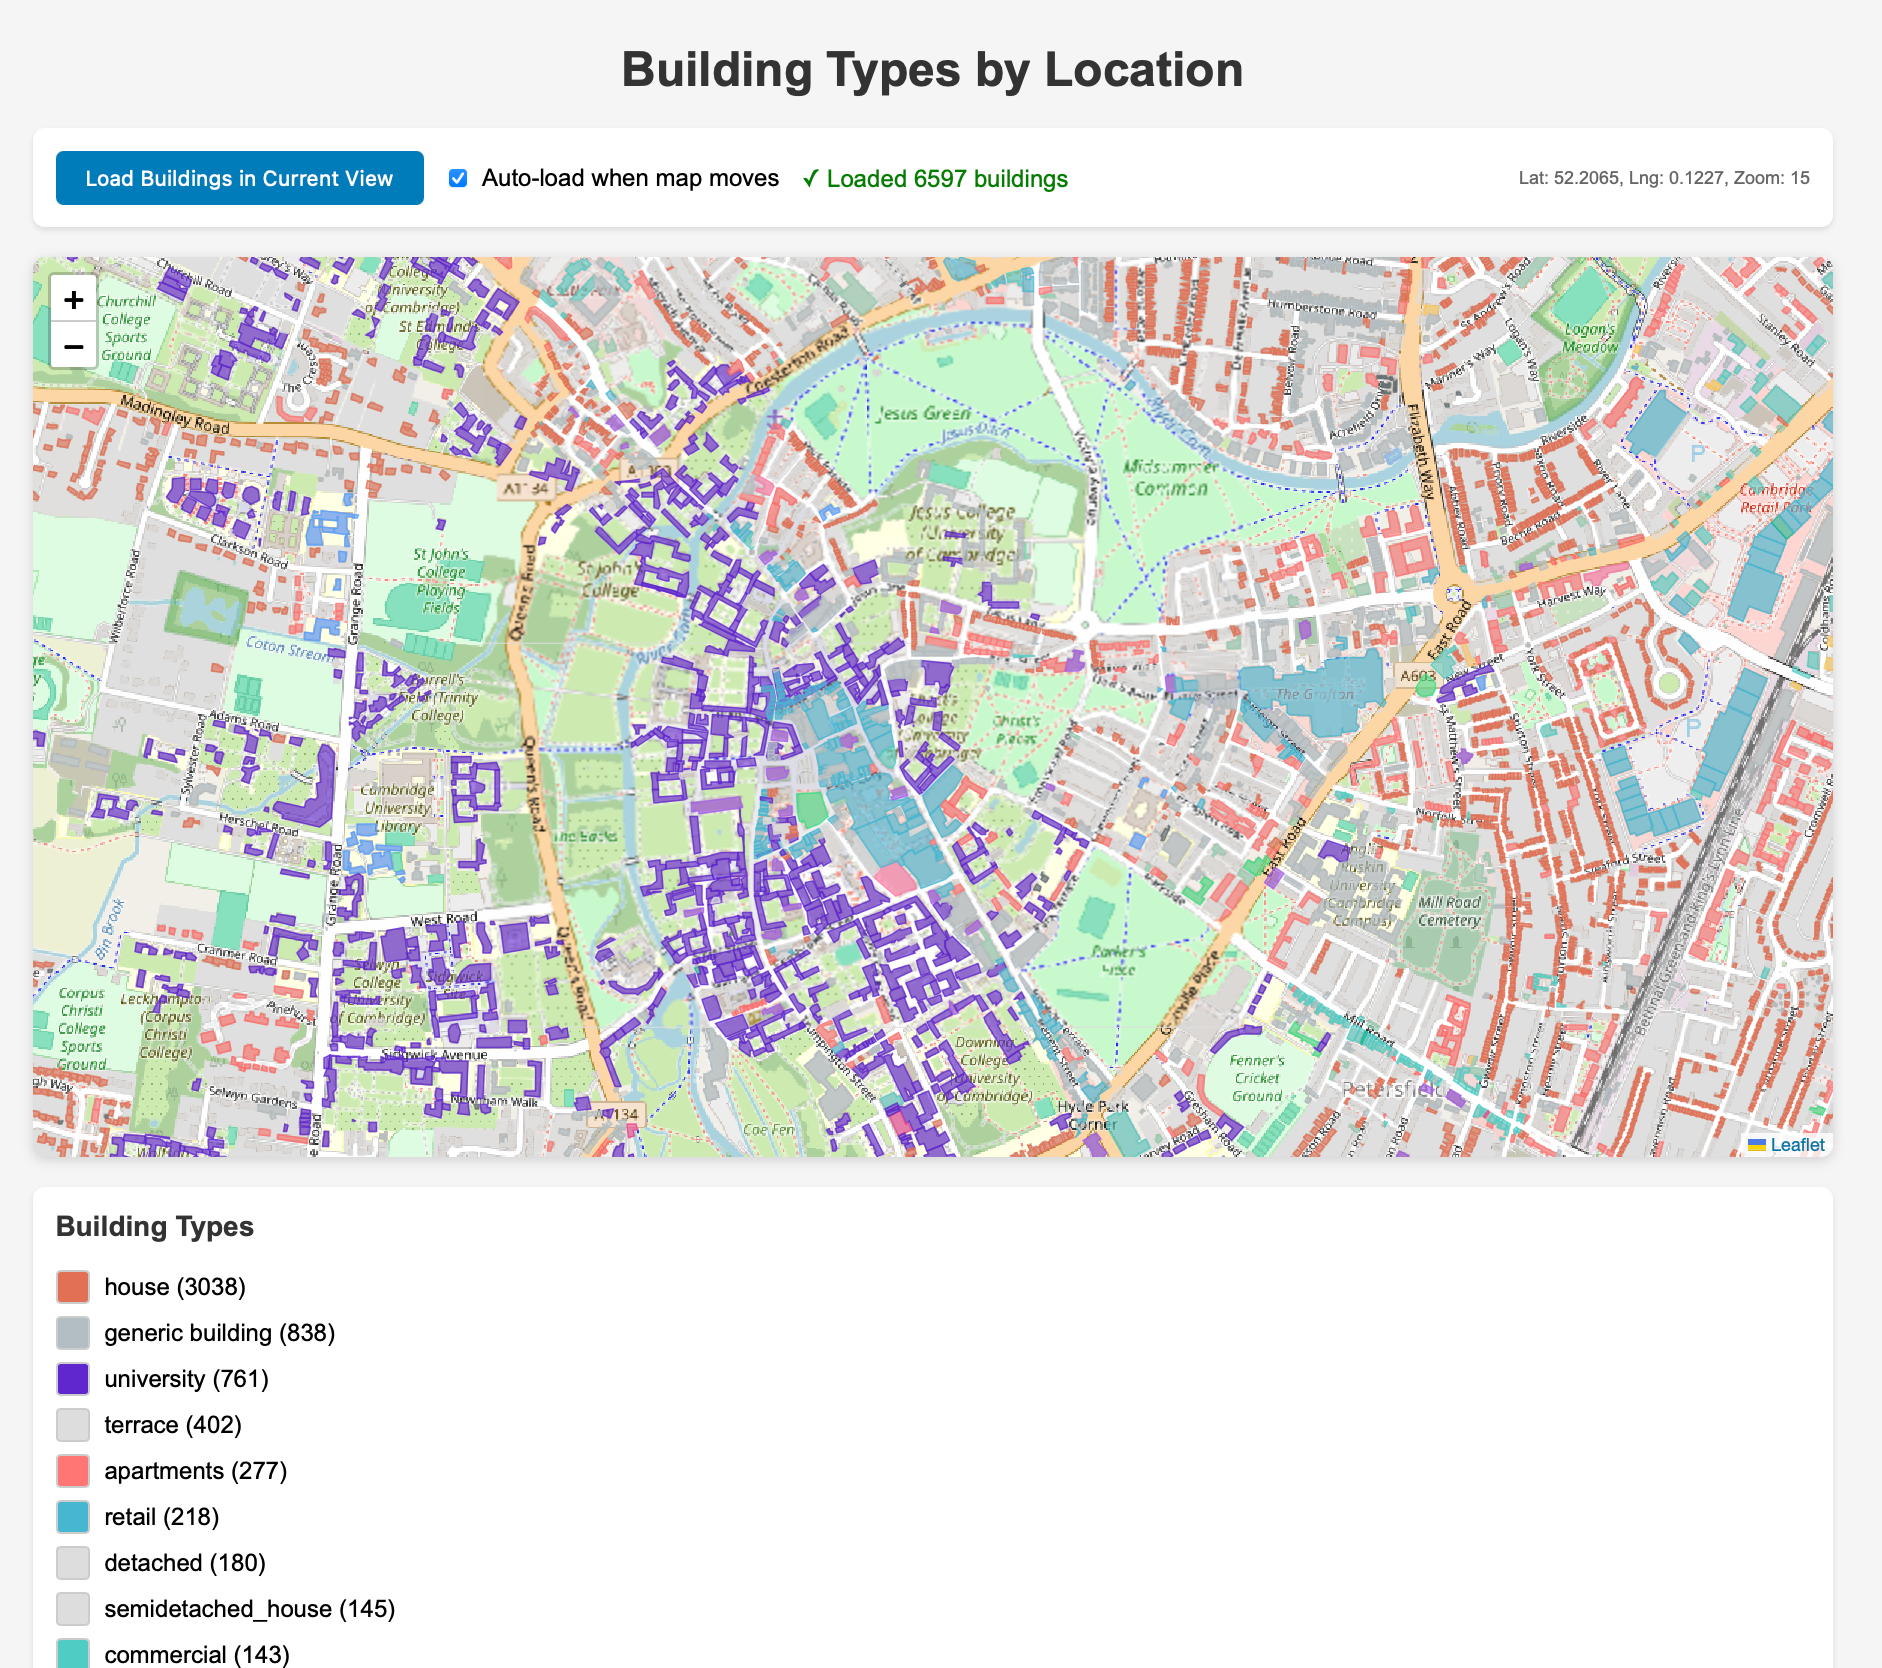
\includegraphics[width=0.7\textwidth]{Chapters/AnalysisMedia/OSMTest.png}
    \caption[]{OpenStreetMap data acquisition test}
    \label{fig:OSMTest}
\end{figure}

I also spent some time on the ONS website file store to find data on employment classifications of workers, this was hugely successful I found employment data dating from 2025 to 1980 years which is perfect for my agent generation algorithm


\begin{figure}[H]
    \centering
    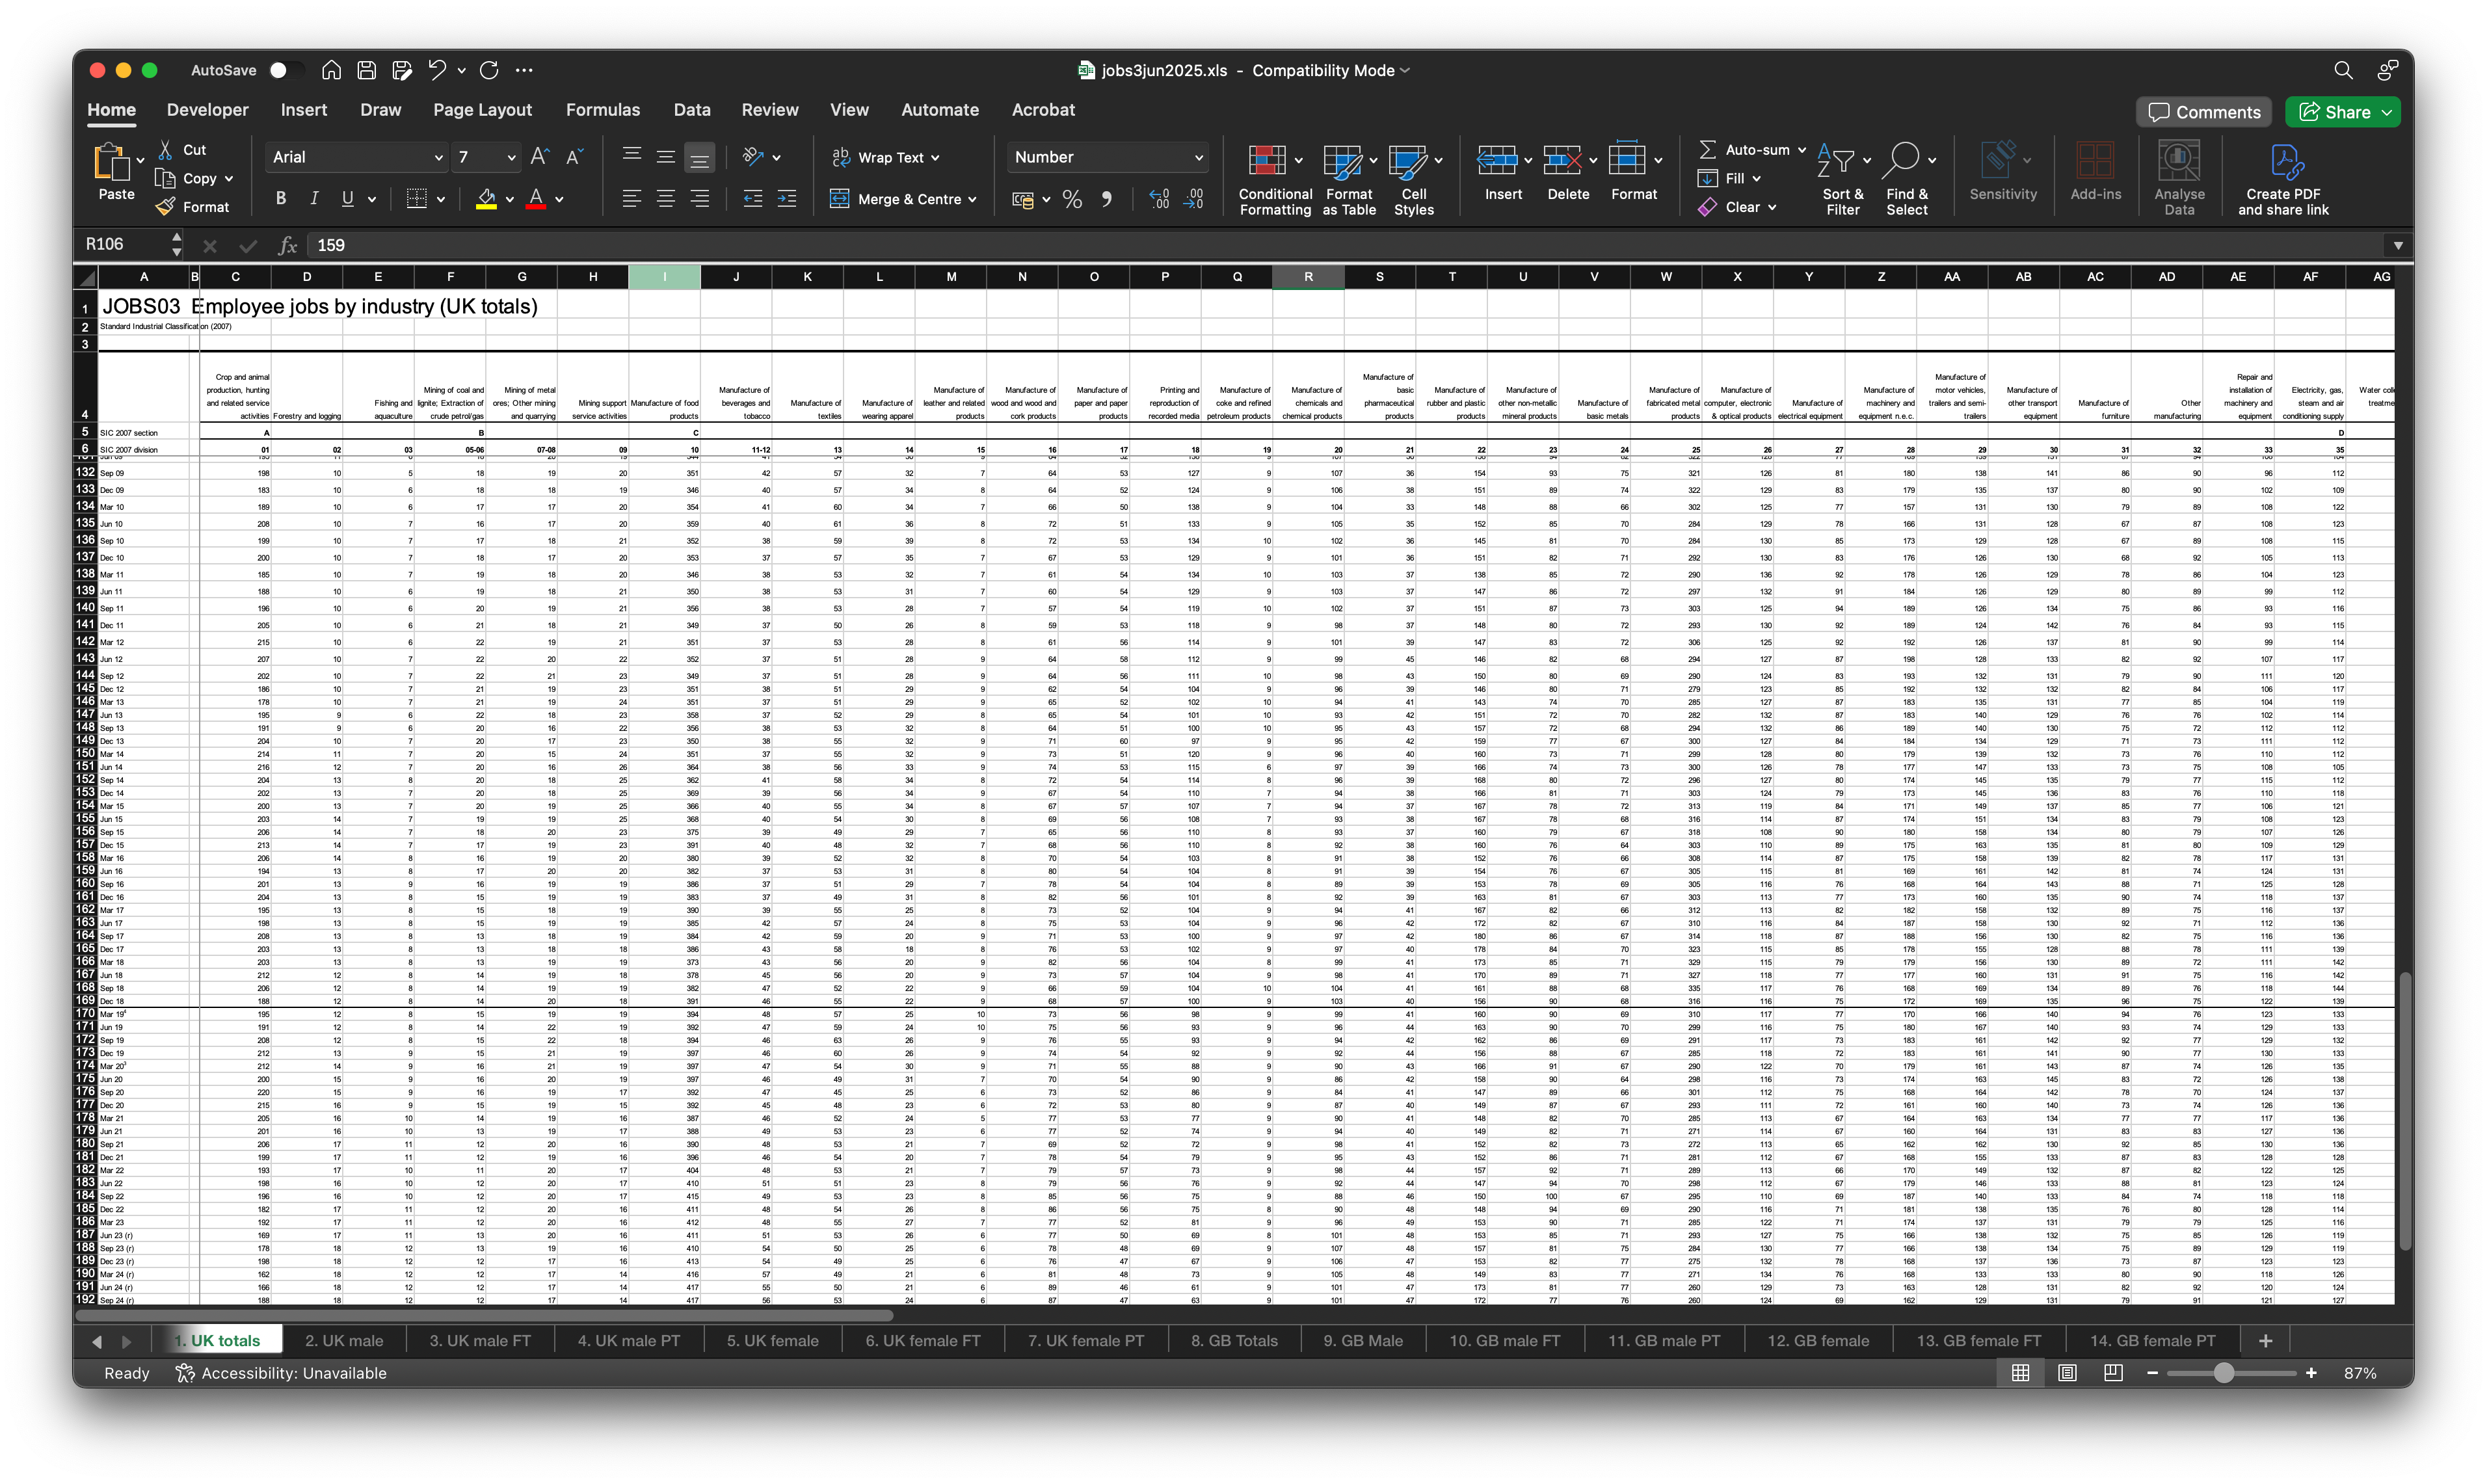
\includegraphics[width=0.7\textwidth]{Chapters/AnalysisMedia/ONSTest.png}
    \caption[]{ONS data acquisition test}
    \label{fig:ONSTest}
\end{figure}

\subsection{Api}
I already have experience using flask to create rich API’s and web socket connections to stream between client and backend software. I was aware that to track every agent movement (~13 bytes per agent x 100,000 agents = 1.3MB) in addition to statistics for each tick was quite a lot of data especially if the user was skipping through the simulation at high speed (resulting in more ticks per second read), I tested a simple client/server interface and was able to achieve over 100 ticks per second (on chrome, firefox and other non chromium browser have much lower WebSocket bandwidths unfortunately), and that was without any optimisation but had excellent network connection between two devices on the same network.
\subsection{Data Visualisation}
to test some data visualisation and some brief physical interaction created a simplistic physics model that could visualise the spread of disease in a 3d model. This also gave me the opportunity to test some biological reporting tools such as R rate (I still have some work to do here however).

\begin{figure}[H]
    \centering
    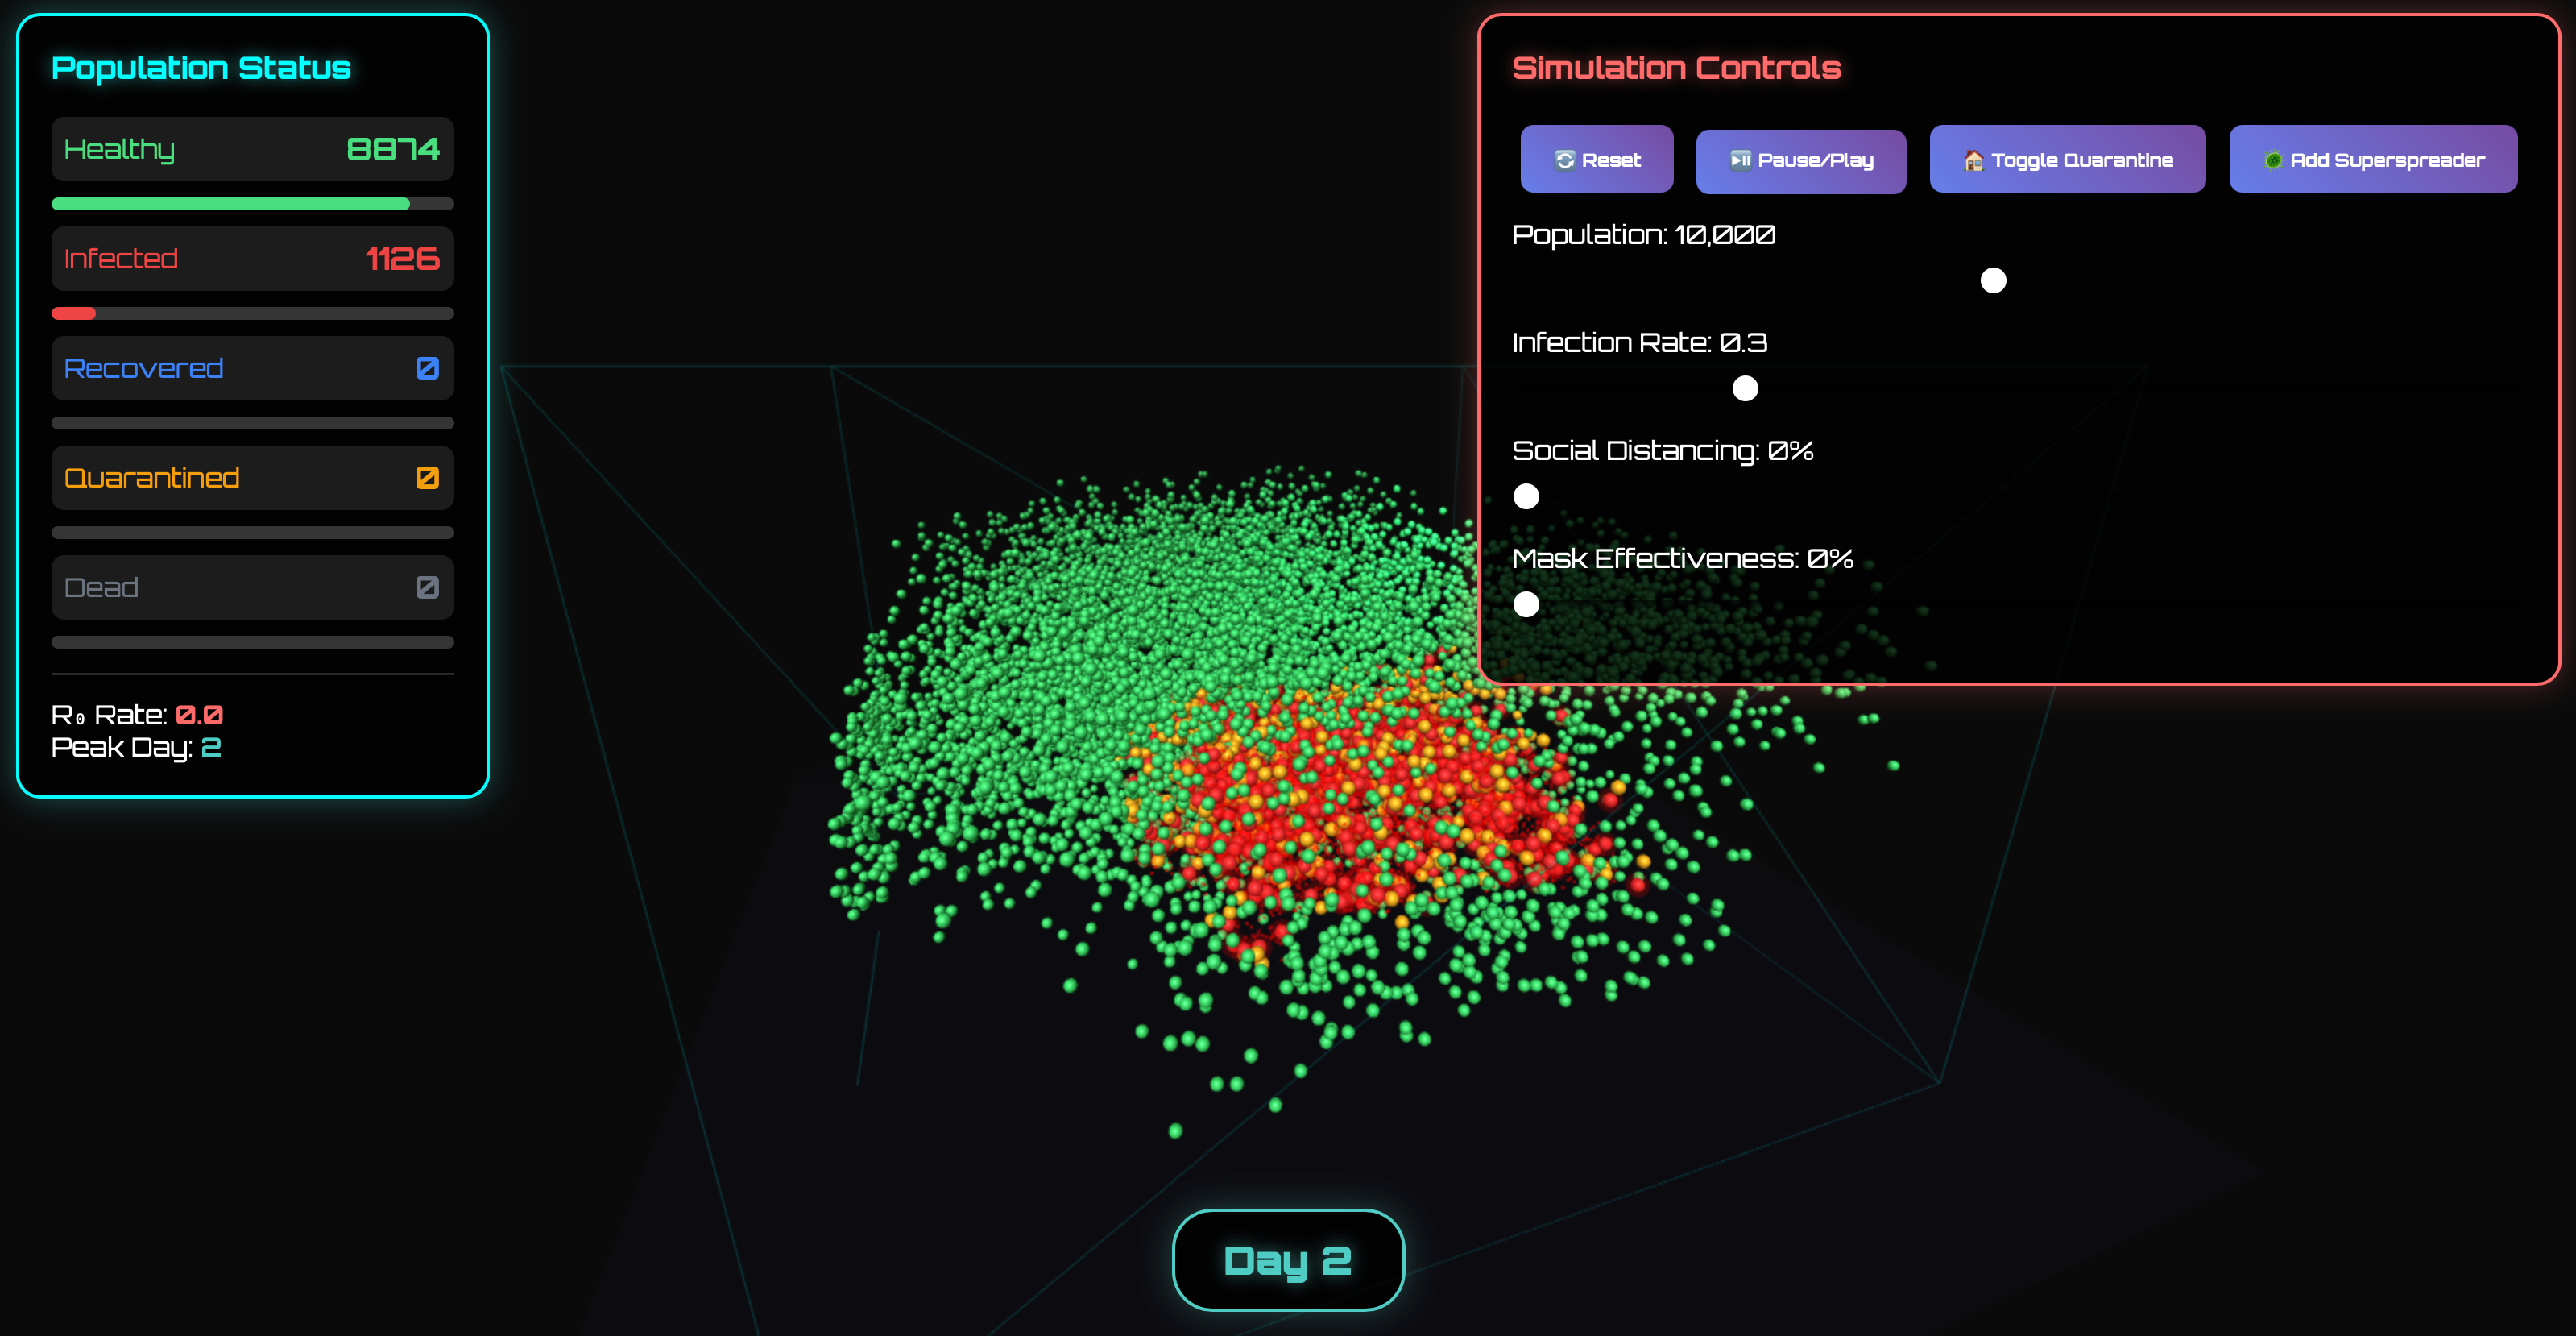
\includegraphics[width=0.7\textwidth]{Chapters/AnalysisMedia/3DTest.png}
    \caption[]{3D visualisation test}
    \label{fig:3DTest}
\end{figure}

\subsection{Simulation Server}
With such a large number of agents being simulated I was aware that this would have a heavy compute premium, especially since I wanted the simulation to simulate at a rate of 1 virtual day per couple of real world seconds. Unsure whether my preferred programming language of python would be suitable I created a simple ‘benchmark’ which loaded 100,000 agents and 50,000 nodes into memory and simulated them each being assigned a new location and potentially a new state (infected, cured etc) per tick.
In my first python iteration which used large lists for all data, the data calculated at 1.5 Ticks per second which was far too slow to be useful, bearing in mind this benchmark was very simplistic and purely focused on randomising movement for each agent this was glacial.
To try and remain within the python ecosystem I looked to implement python numba to handle such large variables. I found that this tool hugely improved the performance (to 211 ticks / s) but hugely increased system memory usage (4x non numba) which would make my backend system non scalable, the codebase also became lightly less readable / maintainable
Concerned with low performance (even with the numba addition) I decided to recreate my program in C\# - a compiled language. I found an immediate, huge improvement to 1599 Ticks per second with code that was functionally the same differing only in language. Whilst it might therefore seem sensible to fully work within C\# I am far more familiar with python tooling for data analysis and Api functionality

\subsection{Data Storage and streaming}
With my dual system of python API / analysis layer and C\# simulation layer planned I needed to test a method to stream data between the two
Initially I thought to store every simulation movement and path trace etc inside a Postgres DB however this resulted in my device resource utilisation spiking and C\# ticks per second falling to 12 due to the heavy read/write penalty of interacting with so many queries, even with batch processing I only gained a couple more Ticks per second. Testing with python caused the Ticks/s to fall so low my 10minute run only parsed 3 ticks, completely unusable.
With database writing written off (at least for main data streaming) I instead decided to test direct socket connections between python and C\# and found much greater success
\section{Success Criteria for Project}
To reflect on my progress I have formed some firm success criteria that I must meet at various stages of my software development
\subsection{Platform Access}
\begin{enumerate}
    \item Users can access the website on any internet connected device
    \item Users log in to the portal and establish a connection with backend end compute servers
    \item Users can view previous simulations, browse a library of examples / other users published simulations or create a new one
\end{enumerate}
\subsection{Simulation Setup}
\begin{enumerate}
    \item Users can select a geographic area for the simulation to run on from a map of the world. Area size can range from neighbourhood to large city
    \item Users can generate a synthesised populated of up to 100,000 people
    \item Users can automatically utilise statistical data to allocate population with roles and behaviours
    \item Users can generate disease(s) to be used in simulations
\end{enumerate}

\subsection{Disease Spread Simulation}
\begin{enumerate}
    \item Simulation runs in ticks (lasting e.g. 30 minutes each)
    \item Simulation accurately models disease progression through SEIR compartments for each agent
    \item Each tick agents are moved around the map based on their routine, job, and behaviours
    \item Disease spread is then calculated based on agents’ health stats and disease transmissibility (R rate) data if applicable
\end{enumerate}

\subsection{User Interaction}
\begin{enumerate}
    \item Users can pause, resume and scrub forward/background through the simulation timeline
    \item Users can apply a various of mitigations such as closing buildings, routes and enforcing policies such as self-isolation and mask wearing
\end{enumerate}

\subsection{Output and Visualisation}
\begin{enumerate}
    \item The simulation streams real time data to the client’s browser and stores data in a database for post simulation analysis
    \item A live3d map of all locations and agents fills the user’s view
    \item Supporting statistics (infection spread curves, recovered, susceptible etc) are displayed around
    \item Users receive non-technical, intuitive explanations of outcomes via tooltips or guided UI messages.
\end{enumerate}

\subsection{Simulation Speed}
\begin{enumerate}
    \item Simulation must run at minimum speed of 1 simulated day per real time second (when running one dedicated simulation)
    \item System can handle 100,000 agents and 20,000 nodes as an expected data set
    \item Data storage and retrieval latency remains under 2 seconds from client request -> visualisation
\end{enumerate}

\subsection{User Interface}
\begin{enumerate}
    \item  Interface should be intuitive and can be used by a non-expert with minimal training (<5minutes)
    \item Results can be easily interpreted without expert knowledge in industry
    \item Controls are well placed and responsive
    \item Colour, icon, size and placement are used to provide visual hierarchy
\end{enumerate}

\subsection{Accessibility}
\begin{enumerate}
    \item Software has full audio descriptions of any visual functions to provide ease of use for those with visual impairments
    \item Bold Contrast on all interface options
    \item Software functionals on all major browser engines (Chromium, Webkit [safari], Gecko [Firefox])
\end{enumerate}

\subsection{Robustness}
\begin{enumerate}
    \item  System validates all user input without crashing
    \item Calculation / system overloads are gracefully handled with a server refresh and simulation reload
\end{enumerate}

\subsection{Maintainability}
\begin{enumerate}
    \item Whilst an academic project, all code should be well maintained on GIT, issues tracked, Formatting standards upheld and documentation robust
    \item Software hosting process is documented, and code is designed with ‘zero vendor lock in’ and can be easily self-hosted
\end{enumerate}
\subsection{Validation}
\begin{enumerate}
    \item Model outputs are tested against real world result data from epidemics / pandemics to ensure accuracy (within the range expected for a semi-random disease spread)
    \item Should aim for Positive feedback to be received from multiple industry experts
\end{enumerate}
\section{Initial Design Considerations}

Having researched a variety of methods to display user information and complete my simulation I am currently working to this technical stack (from user facing to simulation):
\begin{itemize}
    \item \textbf{Frontend:} Vue Js for dynamic content rendering
    \item \textbf{Backend:} Python Flask API for data handling and simulation control, C\# for the simulation engine
    \item \textbf{Database:} PostgreSQL with PostGIS extension for spatial data storage
    \item \textbf{Hosting:} potentially Docker containers for deployment, potentially on a cloud platform like AWS or DigitalOcean, alternatively can fully self-host
\end{itemize}

This combination of technologies allows me to full utilise Object Orientated Programming (OOP) techniques to create a modular, maintainable codebase that can be easily extended in the future. The use of Python and C\# allows me to leverage the strengths of both languages, with Python handling simulation control and data analysis while C\# provides high performance for the simulation engine. The PostgreSQL database with PostGIS will enable efficient storage and retrieval of spatial data, which is crucial for simulating disease spread in a city / urban environment.

\subsection{UML Class Diagram}
\begin{figure}[H]
    
\begin{center}
\begin{tikzpicture}

  \begin{umlpackage}[x=0,y=0]{SimulationSystem}

    % Class: Agent
    \umlclass[x=0, y=0]{Agent}{
      - Name : String \\
      - Health : Float \\
      - Status : String \\
      - Role : Roles \\
      - Home : Node \\
      - Workplace : Node \\
      - Location : Node
    }{}

    % Class: Node
    \umlclass[x=6, y=0]{Node}{
      - Type : String \\
      - Capacity : Int \\
      - Location : String \\
      - CurrentOccupants : Agent[]
    }{}

    % Class: Roles
    \umlclass[x=6, y=-5]{Roles}{
      - Type : String \\
      - StartTime : Time \\
      - LunchBreak : Time \\
      - EndTime : Time \\
      - Priority : Int
    }{}

    % Class: Disease
    \umlclass[x=0, y=-5]{Disease}{
      - Name : String \\
      - DeathRate : Float \\
      - InfectionRate : Float \\
      - Colour : String
    }{}

    % Class: Simulation
    \umlclass[x=3, y=-10]{Simulation}{
      - Agents : Agent[] \\
      - Nodes : Node[] \\
      - Roles : Roles[] \\
      - Disease : Disease
    }{}

    % Class: Account
    \umlclass[x=3, y=-15]{Account}{
      - Name : String \\
      - Email : String \\
      - Password : String \\
      - Simulations : Simulation[]
    }{}

    % Associations
    \umluniassoc{Agent}{Node}       % Home
    \umluniassoc{Agent}{Node}       % Workplace
    \umluniassoc{Agent}{Roles}
    \umluniassoc{Node}{Agent}    % CurrentOccupants
    \umluniassoc{Simulation}{Agent}
    \umluniassoc{Simulation}{Node}
    \umluniassoc{Simulation}{Roles}
    \umluniassoc{Simulation}{Disease}
    \umluniassoc{Account}{Simulation}

  \end{umlpackage}

\end{tikzpicture}
\end{center}
    \caption{UML class diagram of the disease simulation system.}
    \label{fig:umlDiagram}
\end{figure}

\subsection{Tick Sequence}
The fundemantal time span of my simulation is a 'tick' which represents a period of time in which the simulation runs and agents can move, interact and change state. The tick sequence is as follows:
\begin{enumerate}
    \item \textbf{Agent Movement:} Each agent moves to a new location based on their routine and the current state of the simulation. This movement is influenced by their role (e.g., student, worker) and the locations of buildings in the simulation.
    \item \textbf{Disease Spread Calculation:} After all agents have moved, the simulation calculates the spread of disease based on the current state of each agent and the disease profile. This includes determining which agents become infected, recover, or remain susceptible.
    \item \textbf{State Update:} Each agent's state is updated based on the disease spread calculation. This may involve changing their health status (e.g., from susceptible to infected) and updating their health statistics (e.g., R0, recovery rate).
    \item \textbf{Data Storage:} The current state of the simulation, including agent locations and health statistics, is stored in the database for later analysis. This allows users to review the simulation results and visualize the spread of disease over time.
    \item \textbf{User Interaction:} Users can interact with the simulation by pausing, resuming, or scrubbing through the timeline. They can also apply interventions, such as closing buildings or enforcing policies, which will affect the next tick's agent movement and disease spread.
\end{enumerate}

Choosing the duration of a tick is a difficult balancing act as i want to maximise simulation precision whilst also maintaining acceptible simulation speed. For example a tick time of 1minute would allow for a huge number of agent interactions and an excellent 'slow motion' effect for the viewer however would take much longer to compute, inversely a tick duration of an entire day woudl result in missing the nuance of E.g. going to collect a meal and interacting with other agents in the same venue. I have therefore settled on a tick duration of 30 minutes which allows for a good balance of agent interaction and simulation speed. This duration allows for enough time for agents to move around, interact with others, and for the disease to spread realistically, while still being fast enough to keep the simulation engaging and responsive to user input. Should a user wish to view the simulation at a high speed each day will only involve 48 ticks (a week would be 336 ticks) which my testing found to be a quick computation time enabling multi month and year long simulation to be run in minutes rather than hours.







\chapter{Documented Design}
\chapter{Technical Solution}
\chapter{Testing}
\chapter{Evaluation}
\chapter{References}
\printbibliography[heading=bibintoc, title={Bibliography}]

\end{document}